\documentclass[11pt]{article}

\usepackage{hyperref}
\usepackage{listings}
%for dotex
\usepackage[pdftex]{graphicx}
\usepackage[pdf]{graphviz}
\usepackage[boxed]{algorithm2e} %end for dote
\usepackage{color}

% "define" Scala
\lstdefinelanguage{scala}{
  morekeywords={abstract,case,catch,class,def,%
    do,else,extends,false,final,finally,%
    for,if,implicit,import,match,mixin,%
    new,null,object,override,package,%
    private,protected,requires,return,sealed,%
    super,this,throw,trait,true,try,%
    type,val,var,while,with,yield},
  otherkeywords={=>,<-,<\%,<:,>:,\#,@},
  sensitive=true,
  morecomment=[l]{//},
  morecomment=[n]{/*}{*/},
  morestring=[b]",
  morestring=[b]',
  morestring=[b]"""
}

\lstset{ %
    language=scala,
    identifierstyle=\textbf
}

\title{Activity Trail Design}
\author{Maxim Noah Khailo}
\begin{document}
\maketitle
\section{Purpose}

We need to track all important activity of the system, both machine and human so that
our customers can keep track and organize their business.

\section{Forces}

Forces are problems we have to balance.

\begin{itemize}
    \item Activity is both human and machine.
    \item Machine activity can lead to human activity and vice versa.
    \item The information for each activity needs to be viewable. 
    \item You can view activities from multiple perspectives.
\end{itemize}


\section{Data Structure}

The following data structure design is motivated by the fact that we want to linearize 
activities along many dimensions. It is composed of two parts, activities and trails along dimensions. 

Each activity belongs to many trails. A trail belongs to a dimension. A trail is implemented
as a doubly-linked list where each node in the list is called a Connection. 

Each Connection, connects the activity to the trail.

\newpage
\subsection{Activity}

An activity tracks changes to state made by both the computer and human actors.

We use the term Activity here instead of Event. Though you can think of them as the same 
thing. 

\begin{lstlisting}
    case class Activity(
        id: Id, 
        type: Type, 
        data: Json, 
        created: Instant)
\end{lstlisting}

One requirement is that the activity stores all data needed to visualize and compute on that activity in the data field. 
The type is used to understand how to decode the json for visualization.

An activity object is also immutable since it tracks changes to state but is NOT state.

\subsection{Dimensions and Trails}

So what are dimensions? Dimensions are a collection of activity trails. 

\begin{lstlisting}
    case class Dimension(
        id: Id, 
        name: String, 
        description: String)
\end{lstlisting}

For example, we can look at activities for a customer. So we can have a \emph{customer\_activity}
dimension which will have a head activity that contains the customer.id in the json.

Another example, we may want to look at activities for an order. So we can have an \emph{order\_activity}
dimension which will have a head activity that contains the order.id in the json.

Another example, we may want to look at all activities by an admin. So we can have an \emph{admin\_activity}
dimension.

Another example, watch list is just another activity trail. So we would have a \emph{watched\_activities}
dimension. 

\subsection{Connection}

Each activity exists in many trails. The trails are modeled as doubly-linked lists where
a node in the list is called a Connection. It connects an activity to a trail.

\begin{lstlisting}
    case class Connection(
        id: Id, 
        dimension: Id, 
        activity: Id, 
        previous: Id, 
        next: Id, 
        tail: Id,
        trailId: Id,
        data: Json)
\end{lstlisting}

Each activity is connected to a trail by a connection creating a doubly linked list. Each
trail belongs to some dimension. 

Each list has a tail activity and the tail activity has a connection where
the \emph{previous} points to the last activity in the trail and the \emph{next} points to the oldest activity (the head).

Each connection points to the tail for optimization purposes. We can create an
index on the tail id to do quick queries based on the dimension.

Each connection also has a trailId which is used to quickly query for all connections grouped
by that id. The use case is if a dimension represents activity for a type of object, say customer,
where we can put the customer id as the trail id. 

Also each connection can have data. For example, if we model a notification list as a trail in the
watched\_activities dimension, we can model whether a user seen the activity by storing
that state in the data section on a connection.

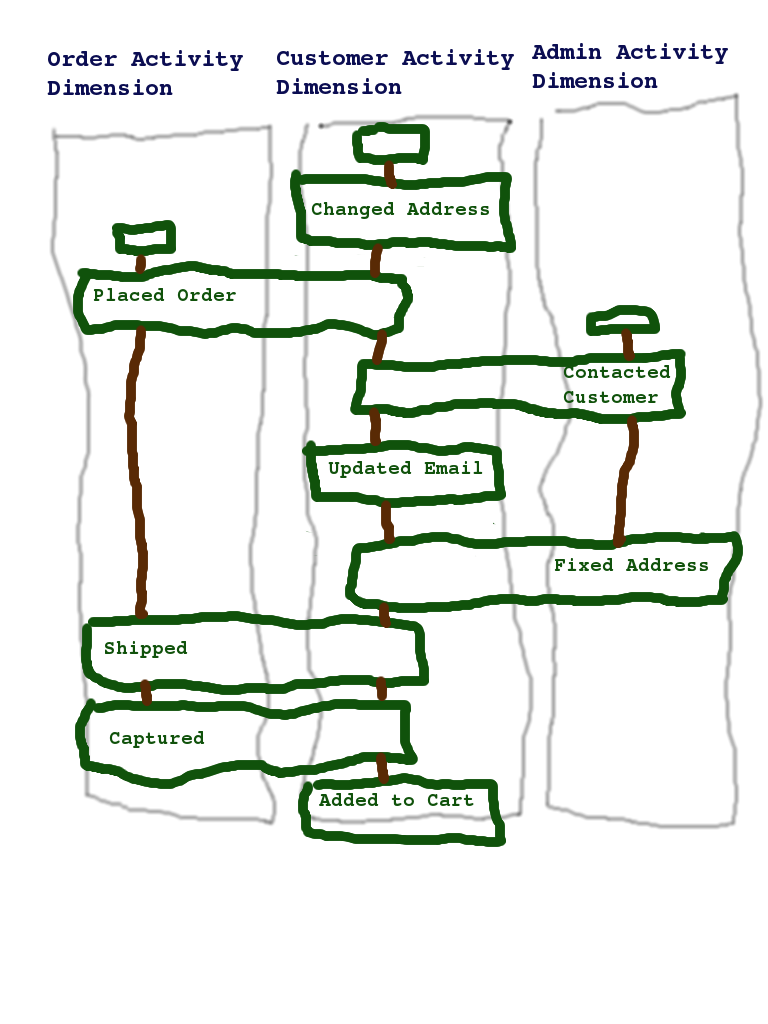
\includegraphics[scale=0.40]{dimension}

\section{Innovative UI}
\subsection{Visualization}

One requirement for an activity is that all the data necessary for visualization is stored
in the JSON. While this will increase the amount of data stored, it will improve performance
in the UI by reducing the amount of queries. 

\subsection{Navigation}

One huge advantage to the data structure is that you can easily navigate it along multiple
dimensions efficiently. This provides interesting UI options in the future when you need
to jump from one view of activities to another.

\section{Implementation}


\subsection{How are Activities Generated?}

Activities themselves, since they are targeted towards end user will mostly be generated
in phoenix and inserted into one activity table. Some activities might be able to 
be created via kafka consumers but phoenix usually has all the metadata on hand
to create an activity.

\subsection{How are Activities Connected to Trails?}

Activities are connected to a trail in a dimension by many Kafka consumers. The consumers
will listen to the activity stream and then connect the activity to a trail.

For example, we will have a notification consumer which will take an activity, check who
is watching the object that activity tracks and add it to the user's notification activity trail.

Magical.

\subsection{Diagram}
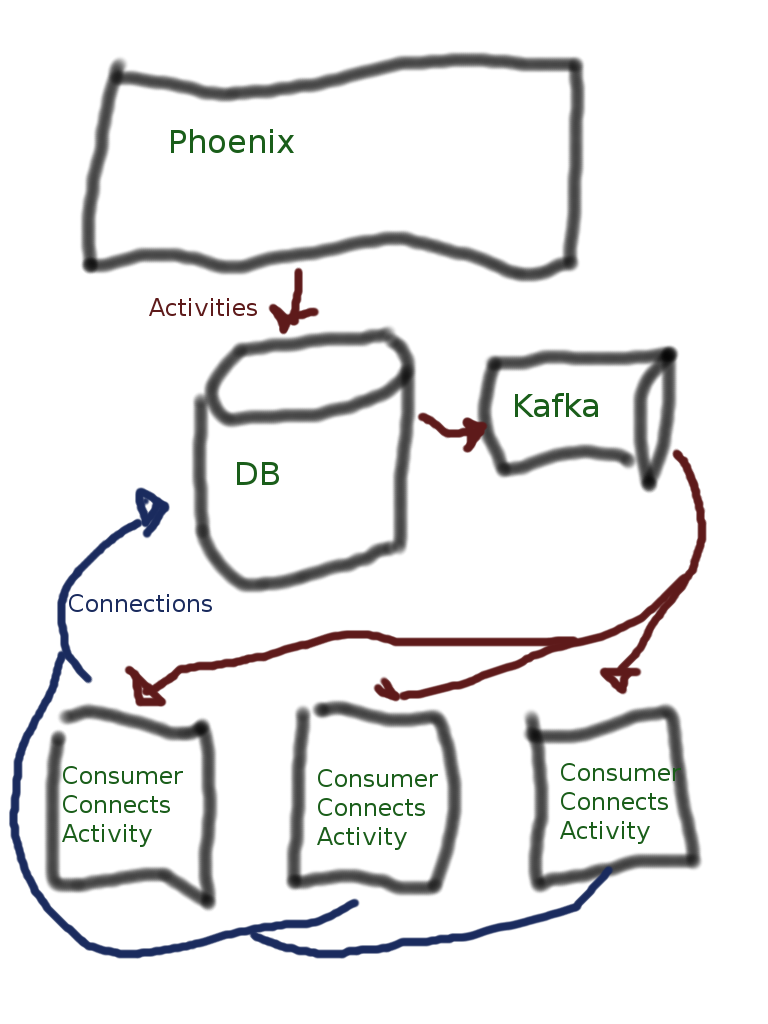
\includegraphics[scale=0.40]{implementation}
\newpage

\section{Discussion}
\subsection{Pros}
\begin{enumerate}
    \item Performance. Cachable completely in Elastic Search
    \item Simplified UI. Activity trail can use the search api instead of hitting DB.
        We can use existing search infrastructure to filter activity trail.
    \item Simplified schema. DB schema is super simple and extensible as we add more dimensions.
        Otherwise we would have to store nulled ids in columns, or have different tables for
        different trails. 
    \item Sets us up for implementing workflows.
    \item Implementing watch and assignment is easy because of how dimensions work. You can
        watch an order, or a customer, or an admin, etc.
\end{enumerate}

\subsection{Cons}

There are many problems to this design.

\begin{enumerate}
    \item Adding an activity requires adding it to multiple trails in many dimensions. 
    \item Size used is greater because each activity stores all data needed for visualization.
    \item Tracking activity is now explicit. Either phoenix needs changes or we create
           Kafka consumers which look at db changes and create the activity objects.
\end{enumerate}

\end{document}
